\chapter{Introduction}
\label{chap:introduction}

Students studying creative computing, creative technologies, and related fields benefit from learning computer programming in various ways. Firstly, programming expands creative possibilities by enabling more interactive and dynamic work, while also providing the ability to customise or even build entirely new digital tools, removing the constraints of `off-the-shelf' software~\cite{shiffman_learning_2008}. It also supports interdisciplinary practice, equipping students to contribute effectively to projects that merge art, design, technology, and science~\cite{greenberg_processing_2016}. Beyond enhancing creativity, programming education fosters industry-relevant capabilities; graduates who possess coding skills can pursue diverse roles in areas such as visual effects, video games, virtual reality, and interactive media~\cite{carey_skills_2019}. Additionally, literacy in different coding languages can facilitate better collaboration by bridging the gap between artists, developers, and technical specialists, leading to more cohesive and effective project outcomes~\cite{davis_role_2006}.

\textit{Creative computing} refers to the use of computer science and programming as media for creativity, employing algorithms, code, and computational processes to generate digital works such as interactive installations, generative art, or digital music. \textit{Creative technology}, by contrast, highlights the application of emerging platforms and tools that extend traditional artistic practices and enable new forms of hybrid or physical expression, such as virtual and augmented reality, 3D printing, sensors, or wearable devices. Both fields sit at the intersection of art, technology, and human innovation, and both prepare students for rapidly evolving creative industries. While one often encounters the terms used interchangeably, the distinction lies in emphasis: creative computing foregrounds computational techniques as a medium of expression, whereas creative technology foregrounds tools and platforms that expand the possibilities of creative practice~\cite{smu_meadows_school_of_the_arts_differences_2023}.

This study focuses on the pedagogical aspects of creative computing and creative technologies practice---specifically, the approach to programming education that emphasises creating multimedia outputs. Such methods typically employ creative coding and art- or design-oriented curricula and teaching methodologies, often aimed at students in creative fields but also applicable to those in other domains~\cite{yee-king_examining_2020}.

More specifically, this thesis explores Python-based creative computing environments (tools and other software) for education. Python, a high-level programming language, has gained significant prominence due to its simplicity, readability, and versatility~\cite{thomas_pragmatic_2019}. Initially developed by Guido van Rossum and released in 1991, Python's design philosophy emphasises code readability and clear syntax, allowing programmers to express concepts in fewer lines of code than C++ or Java. This efficiency and a comprehensive standard library have made Python a favoured choice among developers across various fields~\cite{processing_foundation_overview_2022}. As the forthcoming chapters demonstrate, the Python language's versatility extends beyond conventional software development, finding substantial applications in creative computing.

In summary, this PhD investigates innovative approaches to enhancing Python programming education by integrating, expanding, and developing new creative computing tools (software) and techniques (creative coding practice). It includes the development of tailored curricula, comprehensive documentation, and a sole-authored book. 

Grounded in peer reviewed journal articles (Quartile 2 or higher), the thesis explores and evaluates the effectiveness of Python-based educational environments and creative coding techniques through empirical research methods. Additionally, artistic works showcased at prominent venues illustrate these tools and techniques' practical applications and creative potential. Findings and insights are further disseminated through presentations at esteemed academic and professional conferences, promoting broader awareness and adoption of these advancements in programming education.

\section{Thesis Presentation}

This PhD thesis employs a hybrid structure combining elements of (primarily) a \textbf{Folio of Advanced Professional Practice} and (secondarily) a \textbf{Thesis by Publication}, as defined in the \textit{Higher Degree by Research Thesis Guidelines}\footnote{~TUA Higher Degree by Research Thesis Guidelines at \url{https://torrens.blackboard.com/bbcswebdav/xid-44216710_1}} set forth by Torrens University Australia. 

The elected format allows for a comprehensive exploration of the PhD topic and new development (and testing) of innovative methods in Python creative computing through bespoke software development, scholarly publications, presentation outputs, and creative works---all completed during the PhD enrolment, which commenced in October 2019 (Appendix \ref{appendix:vuw-candidature}), and forming a coherent and thematic research narrative. This collection of outputs forms the core of the folio, with each marking a significant milestone in the research journey. Collectively, they contribute to the academic discourse surrounding Python programming education that employs creative computing environments, addressing existing gaps in the literature while proposing novel solutions to contemporary pedagogical challenges.

For the reader's convenience, this thesis organises the outputs by type (\nameref{chap:publications}, \nameref{chap:presentation-outputs}, \nameref{chap:creative-works}) and, within each grouping, presents the contents in chronological order to illustrate the research's evolution over time. Where practical and necessary, each output is presented in full, prefaced by a concise introduction that situates it within the broader research narrative. These works span various stages of inquiry, from initial exploration and hypothesis development to detailed studies and practical applications. Central themes are consistently revisited through diverse methodologies and analytical frameworks, reinforcing the study's contributions.

\subsection{Chapter Structure}

This outline provides a high-level summary of the chapters comprising this PhD thesis, using concise chapter descriptions and a diagram (Figure~\ref{fig:thesis-overview}) to offer a conceptual overview of the entire document's contents. The elected structure facilitates a thorough understanding of the core concepts and research journey, and includes dedicated chapters that group folio outputs. Moreover, it accommodates the study's practical implications, significance, limitations, and discussion on potential future directions.

\begin{figure}[htbp]
  \centering
  \setstretch{0.7}
  \begin{forest}
  for tree={
    align=left,
    anchor=west,
    calign=first,
    child anchor=west,
    draw=none, % no cell outlines
    font=\footnotesize,
    forked edges,
    grow'=east,
    l sep=1cm,
    parent anchor=east
  }
  [, phantom
    [\ref*{chap:introduction}.~~\nameref*{chap:introduction}, fill=red!20]
    [\ref*{chap:literature-review}.~~\nameref*{chap:literature-review}, fill=blue!20
      [\nameref{sec:creative-coding-software}, fill=blue!20]
    ]
    [\ref*{chap:software}.~~\nameref*{chap:software} (Thonny-py5mode and accompanying documentation), fill=green!20]
    [\ref*{chap:publications}.~~\nameref*{chap:publications}, fill=orange!30
      [\nameref{sec:no-starch} {[No Starch Press 2021]}, fill=orange!30]
      [\nameref{sec:mtap} {[MTAP 2024]}, fill=orange!30]
      [\nameref{sec:jise} {[JISE 2025]}, fill=orange!30]
    ]
    [\ref*{chap:presentation-outputs}.~~\nameref*{chap:presentation-outputs}, fill=gray!30
      [\nameref{sec:processing.py-creative-coding-with-python} {[Kiwi PyCon X (2019)]}, fill=gray!30]
      [\nameref{sec:processing-python-mode-for-creative-coding-and-teaching} {[Libre Graphics Meeting 2020]}, fill=gray!30]
      [\nameref{sec:creative-coding-with-python-and-processing} {[CC Fest 2021]}, fill=gray!30]
      [\nameref{sec:novel-visualisations-with-python-and-p5} {[Outlier 2021]}, fill=gray!30]
      [\nameref{sec:thonny-+-py5-a-python-3-environment-for-processing} {[Processing Community Day (2021)]}, fill=gray!30]
      [\nameref{sec:generate-svg-for-pen-plotters-using-python} {[CC Fest 2022]}, fill=gray!30]
      [\nameref{sec:demystifying-the-python-processing-landscape-an-overview-of-tools-combining-python-and-processing} {[SIGGRAPH 2022]}, fill=gray!30]
      [\nameref{sec:generative-art-with-python-using-py5-and-bpy} {[PyCon XI (2022)]}, fill=gray!30]
      [\nameref{sec:blender-scripting-for-creative-coding-projects} {[SIGGRAPH Asia 2022]}, fill=gray!30]
      [\nameref{sec:mitigating-ai-misuse-in-introductory-python-courses-with-graphical-programming-tasks} {[PyCon 2025]}, fill=gray!30]
    ]
    [\ref*{chap:creative-works}.~~\nameref*{chap:creative-works}, fill=pink!40
      [\nameref{sec:the-end-of-random-seed} {[exhibited at Between 2021]}, fill=pink!40]
      [\nameref{sec:north} {[exhibited at ADA Network Symposium 2021]}, fill=pink!40]
      [\nameref{sec:south} {[exhibited at Link Conference 2021]}, fill=pink!40]
      [\nameref{sec:relics-u130c8} {[exhibited at Motyf 2022]}, fill=pink!40]
      [\nameref{sec:digital-aquatics} {[published in Processing Community Catalog (2023)]}, fill=pink!40]
    ]
    [\ref*{chap:conclusion}.~~\nameref*{chap:conclusion}, fill=cyan!20
      [\nameref{sec:contribution-to-knowledge}, fill=cyan!20]
    ]
  ]
  \end{forest}
  \vspace{1mm}\caption{Overview of thesis contents and structure}
  \label{fig:thesis-overview}
\end{figure}

\paragraph{\ref{chap:introduction}.~~\nameref{chap:introduction}}
(current chapter) Introduces the thesis by outlining the content structure and describing its context, scope, and significance. It lists the research objectives and questions, laying the groundwork for the key themes explored in subsequent chapters, and provides an introduction to creative coding, programming education, and Python.

\paragraph{\ref{chap:literature-review}.~~\nameref{chap:literature-review}}
Identifies gaps in current research and tools related to creative computing and Python programming education, positioning the work within the broader academic discourse. Given the folio/publication-based framing of this thesis, and to avoid repetition, the literature is distributed across the \nameref{chap:publications} (as part of the journal articles), the \nameref{chap:presentation-outputs}, and, to a lesser extent, the \nameref{chap:creative-works} chapter.

\paragraph{\ref{chap:software}.~~\nameref{chap:software}}
Covers the Thonny-py5mode plugin, outlining its key features, supporting documentation, and the development process, including associated funding and recognition. The \textit{\nameref{sec:jise}} article complements this chapter by detailing the plugin's technical implementation and design rationale. \nameref{chap:publications}, \nameref{chap:presentation-outputs}, and \nameref{chap:creative-works} assess the software's effectiveness and its contribution to the research objectives, while also demonstrating its practical applications and broader capabilities.

\paragraph{\ref{chap:publications}.~~\nameref{chap:publications}}
Presents the collected manuscripts---comprising a sole-authored book and peer reviewed articles published in Q1 and Q2 journals---that together form the scholarly core of the thesis. These works explore both new and existing tools, techniques, and curricula for Python-based creative computing, including results of the user studies conducted as part of this research.

\paragraph{\ref{chap:presentation-outputs}.~~\nameref{chap:presentation-outputs}}
Documents each presentation accompanied by an introduction that outlines its contribution to the thesis and integration into the overall research narrative. Delivered at prominent gatherings, the topics encompass innovative tools, creative coding practices, and teaching methodologies in Python programming that emphasise a focus on creative computing.

\paragraph{\ref{chap:creative-works}.~~\nameref{chap:creative-works}}
Presents a series of creative works developed using Python-based creative coding tools and techniques explored throughout this PhD research. These works have been exhibited at various online and in-person events and featured in published outputs.

\paragraph{\ref{chap:conclusion}.~~\nameref{chap:conclusion}}
Consolidates the research findings, tools, publications, presentations, and creative works, demonstrating how they collectively advance Python programming education through creative computing. Specifically, it highlights the interconnections among these outputs and their broader implications for educational practice, summarises the key findings, articulates the thesis' \nameref{sec:contribution-to-knowledge}, and reflects on the strengths and limitations of the developed tools and techniques. The chapter concludes by outlining future research directions and opportunities for further innovation in Python-based creative computing environments.

\paragraph{\hyperref[appendix:start]{Appendices}}
Collects supplementary material supporting the thesis, including ethics clearance, folio evidence, survey forms, anonymised data, code samples, and other relevant resources. Where applicable, chapter content will cite resources contained within the appendices.

\subsection{A Note on Methodology}

Notably, this thesis does not include a dedicated Methods or Methodology chapter. Following thesis-by-publication conventions, each output in the \nameref{chap:publications} and \nameref{chap:presentation-outputs} chapters---and, to a lesser extent, the \nameref{chap:creative-works} chapter---details its respective method(s)~\cite{denholm_supervising_2007}. The PhD folio is interdisciplinary in nature, spanning digital technology, education, and creative practice across multiple output types. Such a scope necessitates varied methodological framings~\cite{robins_phd_2008}. Accordingly, the thesis situates its methods within the development process rather than fixing them in advance. A linking commentary and concluding chapter synthesise the diverse strands, articulating the evolution of the PhD process as a whole. Moreover, the structure avoids repetition and supports the coherence of the folio/publication thesis format.

\section{Research Context and Significance}
\label{sec:research-context-and-significance}

This PhD argues that an increasing convergence of art, design, and technology has amplified the need for robust programming education tailored to creative disciplines. As technology continues to permeate facets of creative work, the ability to program is a valuable skill that can expand creative boundaries, facilitate interdisciplinary collaboration, and open doors for graduates entering emerging industries. However, teaching programming to students within creative fields can present unique challenges~\cite{carey_skills_2019, davis_role_2006, shiffman_learning_2008}. Creative computing offers a promising approach that invites learners to merge computational thinking with artistic and design-based expression.

Software applications like the Processing\footnote{~\url{https://processing.org}} IDE (Integrated Development Environment) provide creative computing environments for writing code in Java and other languages. While older versions of the Processing IDE can accommodate Python, work on this aspect is now discontinued and ``Python Mode'' (Processing.py) will not operate correctly in current versions. 

Python is a widely used programming language known for its simplicity and versatility~\cite{kaila_changing_2023}; this thesis argues that there remains significant potential for developing new Python-based tools and pedagogical approaches---akin to Processing's---that make coding more accessible, engaging, and aligned with the goals of learners pursuing foundational programming education for eventual entry into creative industries. 

Figure~\ref{fig:venn-positioning} illustrates how this PhD is positioned at the convergence of Creative Coding, Programming Education, and Python. 

\begin{figure}[htbp]
\centering
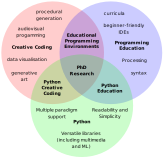
\includegraphics[width=0.7\textwidth]{chapters/chapter01-introduction/venn-positioning}
\captionsetup{width=0.7\textwidth}
\caption{Venn diagram positioning this PhD research. Figure by the author.}
\label{fig:venn-positioning}
\end{figure}

The PhD focus is developing new tools, curricula, and methods that offer students in creative (and even other) disciplines an approachable way to learn \textit{textual programming}\footnote{~Textual programming involves typing lines of code instructing computers to perform tasks} through coding graphical and interactive outputs using Python. As illustrated in Figure~\ref{fig:venn-context}, the research examines the topic from three principal angles:

\begin{figure}[htbp]
\centering
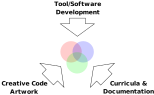
\includegraphics[width=0.7\textwidth]{chapters/chapter01-introduction/venn-context}
\captionsetup{width=0.7\textwidth}
\medskip\caption{Contextualising this PhD research approach. Figure by the author.}
\label{fig:venn-context}
\end{figure}

\begin{enumerate}

\item{\textbf{Tool/Software Development}:} 
Focussing on creating, integrating, and refining Python-based tools, notably the Thonny-py5mode plugin, developed as part of this research to facilitate creative coding practices. Thonny-py5mode is designed to align with the needs of creative disciplines, enabling seamless integration of Python code into artistic processes. Its development emphasises usability and accessibility, striving to accommodate students from varying technical backgrounds to engage with code through programming multimedia outputs.

\item{\textbf{Curricula \& Documentation}:} 
Involving designing new educational materials and curricula tailored to programming education for creative disciplines; this includes comprehensive texts---a sole-authored book and web-based software tutorials---that promote a hands-on, exploratory learning experience aimed at producing graphical and interactive output using Python code. The goal is to bridge the gap between technical programming concepts and creative practice, accommodating a learning environment where students can apply programming in meaningful, artistic contexts.

\item{\textbf{Creative Code Artwork}:} 
Exploring the application of Python-based tools and techniques through the creation of digital art and interactive media, including original artworks exhibited at events and in published catalogues. These demonstrate the potential of the environments and tools explored and developed as part of this research, while also showcasing how programming can inspire creative project outcomes.

\end{enumerate}

The significance of this study lies in its potential to influence programming education for creative fields. It contributes to the growing body of knowledge in creative computing pedagogy, providing educators with new strategies and tools to enhance student engagement and learning outcomes. Moreover, the practical implications of this research extend beyond the classroom, as the tools and techniques developed here can offer new ways to produce code-generated output for a broad range of creative applications, including digital art, design, interactive media, and entertainment.

The subsections that follow provide an essential introduction to \nameref*{sec:intro-creative-coding}, \nameref*{sec:intro-programming-education}, and \nameref*{sec:intro-python}, as contextualised within this PhD. These topics are explored in greater detail in the \nameref{chap:literature-review} chapter, as well as through the outputs presented in the \nameref{chap:publications}, \nameref{chap:presentation-outputs}, and \nameref{chap:creative-works} chapters.

\subsection{Creative Coding}
\label{sec:intro-creative-coding}

Creative coding spans applications like generative art, motion graphics, live coding performances, interactive installations, wearables, and robotics. In education, it engages students in programming through hands-on, interdisciplinary projects that blend art, design, and technology. This approach encourages curiosity, lowers the fear of failure, and makes coding more accessible by connecting it to visual, auditory, and tactile experiences~\cite{bown_creative_2020, caravati_interfacing_2024}.

It is common in creative coding to refer to programs as ``sketches,'' especially within Processing environments. This terminology originates from an analogy with visual arts, where a sketch refers to a rough, initial drawing meant to explore ideas. Processing (created by Casey Reas and Ben Fry in 2001) officially adopted this term (Figure~\ref{fig:processing-ide}) to reflect that coding should be experimental and iterative, much like drawing a sketch~\cite{reas_processing_2014}. 

\begin{figure}[htbp]
\centering
\includegraphics[width=0.8\textwidth]{chapters/chapter01-introduction/processing-ide}
\captionsetup{width=0.8\textwidth}
\caption{Screenshot of the Processing 4.3 IDE. Note the use of ``Sketch'' within the interface. Screenshot by the author.}
\label{fig:processing-ide}
\end{figure}

This aligns with the philosophy of Processing, which encourages users---especially artists and designers---to approach programming with a creative, low-stakes mindset. The term ``sketch'' is used in other creative coding tools and frameworks, including p5.js (a JavaScript version of Processing) and Arduino (microcontroller programming).

Creative coding emphasises creative outcomes over abstract syntax, attracting learners not typically drawn to computer science while engaging students across art, music, and design (and also computing \& information sciences)~\cite{mcnutt_study_2023, wing_computational_2006}. Its adaptability and emphasis on exploration provide an inclusive framework for programming education, supporting varied learning pathways and modes of skill development~\cite{urban_arts_creative_2023}. In addition to introducing core technical skills, creative coding can offer several other benefits:

\paragraph{Engagement and Motivation} Research affirms that creative coding environments can increase student engagement and motivation by situating programming within contexts that feel meaningful and enjoyable. Walsh \textit{et al.} demonstrate how combining craft with block-based coding in Scratch encourages sustained interest and playful exploration~\cite{walsh_crafting_2022}. Dufva highlights how frameworks such as Processing and Arduino stimulate intrinsic motivation by reframing code as a form of creative expression~\cite{dufva_creative_2021}. These findings support broader claims that creative coding projects make the process of learning programming more enjoyable and encouraging~\cite{mccarthy_getting_2015}.

\paragraph{Inclusivity and Appeal to Underrepresented Groups}  
Research increasingly shows that creative coding contexts can broaden participation by engaging groups historically underrepresented in computing. Walsh \textit{et al.} found that arts-integrated coding activities promoted inclusivity among underserved urban youth~\cite{walsh_crafting_2022}; Dufva emphasises feminist and critical approaches that frame coding as a cultural and political practice rather than a purely technical skill~\cite{dufva_creative_2021}. Prominent creative coding communities explicitly promote diversity and inclusion~\cite{long_coding_2023}, such as The Processing Foundation, whose mission statement directly highlights these values~\cite{processing_foundation_processing_2024}.

\paragraph{Lowering Barriers to Entry} Simplified, beginner-friendly environments lower the threshold for participation by reducing technical overhead~\cite{walsh_crafting_2022}. Dufva situates Processing and Arduino as accessible platforms for experimenting with art and code~\cite{dufva_creative_2021}, complementing findings that such environments avoid complex setup, while simultaneously providing a pathway between novice and professional developer tools with features like autocomplete and debugging functionality, thereby facilitating a smoother transition to industry-standard practices and coding environments~\cite{mccarthy_getting_2015,processing_foundation_overview_2022}.

\paragraph{Code Exploration Through Art} Creative coding highlights the intersection of programming, art, and design. As Dufva demonstrates, this bridges a gap between programming and art education, facilitating playful experimentation through live coding, code poetry, and maker practices~\cite{dufva_creative_2021}. Similarly, Walsh \textit{et al.} highlight how students integrated hand-crafted characters into Scratch games, blurring boundaries between craft and computation~\cite{walsh_crafting_2022}. Tools like number sliders and colour pickers encourage inventive tinkering, helping students to intuitively discover new ideas while still writing textual code~\cite{van_rossum_variables_2023}. Some environments, such as Hydra and Visor (Figure~\ref{fig:visor-ide}), include REPL characteristics, providing rapid feedback in response to code edits and additions. Code is entered and executed piecewise in a REPL (read--eval--print loop), meaning the output updates without rerunning the entire program~\cite{jack_documentation_2022, purvis_cjing_2019}.

\begin{figure}[htbp]
\centering
\includegraphics[width=1.0\textwidth]{chapters/chapter01-introduction/visor-ide}
\caption{Visor is a live coding environment for real-time visual performance, bridging the gap between creative coding and VJing. Screenshot from Jack Purvis (2024). Source:~\cite{purvis_visor_2024}.}
\label{fig:visor-ide}
\end{figure}

\paragraph{Building Confidence and Reducing Frustration} Evidence suggests that creative coding builds learner confidence by providing observable, incremental successes and reducing common frustrations, helping maintain learner momentum and reinforcing a sense of accomplishment~\cite{cc2020_task_force_chapter_2021}. Walsh \textit{et al.} found that students reluctant to engage with coding gained confidence through hybrid craft--code projects, while those already interested developed patience and creativity~\cite{walsh_crafting_2022}. Dufva similarly reports that hands-on, low-stakes assignments (e.g., ``human fax machine'' sound-to-drawing tasks) helped students reframe coding as accessible and culturally relevant~\cite{dufva_creative_2021}. Static analysis tools (e.g., linting) and auto-formatting in creative coding environments help students avoid common errors and maintain organised code. Simplified syntax and libraries lower entry barriers, while supportive communities offer resources and guidance to help overcome challenges~\cite{processing_foundation_overview_2022}.

In summary, creative coding offers a dynamic and inclusive approach to programming education that resonates with diverse learners and transcends traditional coding paradigms. Beginner-friendly tools like Processing and p5.js, coupled with supportive communities, foster confidence and inclusivity. This PhD aims to combine these benefits with bespoke Python-based tools and pedagogy.
    
\subsection{Programming Education}
\label{sec:intro-programming-education}

Programming education has long incorporated visual and interactive elements to enhance student engagement and understanding. Turtle graphics, commonly used in computer education during the 1980s and closely associated with the Logo programming language, provided an engaging way for children to interact with programming concepts through visual feedback~\cite{abelson_turtle_1981}.

Developed by Seymour Papert, Cynthia Solomon, and Wallace Feurzeig, Logo's Turtle graphics allowed children to visualise abstract programming ideas by controlling an on-screen ``turtle'' to draw shapes and patterns. This embodied Papert's \textit{constructionist} learning theory: learning by making, where students build knowledge through actively constructing projects. This simple yet powerful approach sought to make coding more accessible and enjoyable, promoting problem-solving skills in a creative way. Over time, Turtle graphics evolved through various versions and adaptations of Logo~\cite{solomon_history_2020}.

Python's standard library includes a Turtle graphics module inspired by Logo's. The module allows users to control turtles in a 2D space (Figure~\ref{fig:python-turtle}) and remains a popular tool for beginners to learn programming fundamentals using Python's syntax and data structures~\cite{nanavati_pythons_2020, vidal_duarte_when_2017}.

\begin{figure}[htbp]
\centering
\includegraphics[width=0.8\textwidth]{chapters/chapter01-introduction/python-turtle}
\captionsetup{width=0.8\textwidth}
\caption{A simple square drawn using Python's Turtle graphics library, demonstrating basic commands for movement and rotation. Screenshot by the author.}
\label{fig:python-turtle}
\end{figure}

Processing was among the first programming environments explicitly developed for creatives---artists, designers, and others in related fields---emphasising accessibility to programming as a medium for visual expression. Unlike many earlier programming environments focused on visual output, Processing was purpose-built to meet the creative community's needs, streamlining the process of transforming artistic concepts into code and, ultimately, code into multimedia outputs~\cite{reas_modern_2018}.

Several Processing variants have appeared since the release of the (Java-based) original, each designed to extend the Processing concept into different programming environments and languages, including p5.js (JavaScript), JRubyArt (Ruby), and Processing.py (the now outdated Python mode), among others~\cite{wikipedia_processing_2025}.

Processing has significantly impacted programming education, inspiring learners to see coding as a technical skill \textit{and} a medium for creative expression. There is a wealth of books, reference materials, and resources available for Processing and its variants, making it one of the most well-documented creative coding initiatives. As of writing, the Processing website lists 36 books covering topics from programming generative art to data visualisation, many with an introductory programming focus~\cite{processing_foundation_books_2024}. 

Several educational websites use Processing environments to teach programming fundamentals, often within a creative coding context, including 
\href{https://thecodingtrain.com}{The Coding Train}, \href{http://funprogramming.org}{Fun Programming},
\href{https://happycoding.io}{Happy Coding}, \href{https://imaginary-institute.com/}{The Imaginary Institute}, and substantial parts of Khan Academy's \href{https://www.khanacademy.org/computing/computer-programming}{ ``Computer Programming''} section. Strive, an EdTech company, leverages a Processing-based environment to teach mathematics, science, and other subjects through code~\cite{strive_math_editor_2025}.

At this point, it is important to reiterate that \textit{visual programming} languages, as opposed to \textit{textual} programming languages, fall outside the scope of this PhD topic. For instance, Scratch is a notable visual programming language developed in the early 2000s, with the primary goal of making programming accessible, particularly for young learners. It enables them to create stories, games, and animations through an intuitive block-based coding interface (Figure~\ref{fig:scratch-editor})~\cite{mit_media_lab_scratch_2024}. The Scratch community has encouraged a culture of sharing and remixing projects, significantly contributing to its widespread adoption. Its popularity stems from the simplicity of its drag-and-drop coding interface, which promotes experimentation and iterative learning~\cite{resnick_scratch_2009}. Its success has established Scratch as one of the most widely used tools for introducing young learners to programming and computational thinking, influencing the creation of other block-based educational programming environments such as Snap! and Blockly~\cite{marji_learn_2014}.

\begin{figure}[htbp]
\centering
\includegraphics[width=1.0\textwidth]{chapters/chapter01-introduction/scratch-editor}
\caption{The Scratch editor's block-based interface, where users create programs by stacking visual code blocks to form logical sequences. Screenshot of the Scratch web app by the author. Source:~\cite{mit_media_lab_scratch_2024}.}
\label{fig:scratch-editor}
\end{figure}

However, while Scratch may be highly effective for introducing programming, particularly to younger learners, textual programming environments such as Processing are arguably better suited for students ready to engage with more complex concepts and develop skills more closely aligned with real-world programming practices~\cite{ruf_scratch_2014}. The PhD aim is not to explore the merits of either approach (block-based vs textual), as the elected focus is Python.

\subsection{Python}
\label{sec:intro-python}

Python's readable syntax and expressiveness have contributed to its extensive use in industry and education. Unlike languages such as C++ or Java, which often require verbose implementations, Python allows for more concise expression of programming concepts~\cite{ma_you_2021}; it is a versatile, general-purpose language~\cite{matthes_python_2023}. Unlike Processing, it does not include a purpose-built IDE for creative coding or built-in functions intended explicitly for multimedia output. However, Python does offer a vast ecosystem of libraries available on PyPI\footnote{~\url{https://pypi.org}} (Python Package Index) and elsewhere, which can extend Python's capabilities for multimedia projects.

PyPI serves as the official repository for Python packages~\cite{python_software_foundation_pypi_2024}. It is the primary platform for sharing Python packages/libraries and the default source for downloading and installing them. In Python, the terms \textit{libraries} and \textit{packages} are often used interchangeably, though there is a distinction. Regardless, to avoid unnecessary details here, it is enough to know that PyPI primarily hosts packages that can encapsulate libraries. Tools like PIP, Python's standard package manager, connect to PyPI to fetch and install the packages users require.

Table \ref{tbl:python-multimedia-libs} highlights some of the most prominent PyPI multimedia packages, all of which one could employ for creative coding projects. The tabulated data is sourced from PyPI Stats: a platform that removes the need for users to directly query raw download records via Google BigQuery~\cite{flynn_about_2024}, that provides aggregate download figures for Python packages hosted on PyPI. Note that Tkinter, a widely used GUI library known for its simplicity and ease of use~\cite{moore_python_2021}, is part of Python's standard library and therefore not distributed via PyPI. As such, the table does not report download data for it.

\begin{table}[!htbp]
  \centering
  \fontsize{9.75pt}{10pt}\selectfont{}
  \renewcommand{\arraystretch}{2}
  \begin{tabular}{
    >{\raggedright\arraybackslash}p{\dimexpr 0.2\linewidth-2\tabcolsep}
    >{\raggedright\arraybackslash}p{\dimexpr 0.2\linewidth-2\tabcolsep}
    >{\raggedright\arraybackslash}p{\dimexpr 0.4\linewidth-2\tabcolsep}
    >{\raggedright\arraybackslash}p{\dimexpr 0.2\linewidth-2\tabcolsep}
  }
    \hline
    \textbf{Category} & \textbf{Name} & \textbf{Description} & \textbf{Downloads (October 2024)} \\
    \hline

    \multirow{3}{=}{3D Graphics} 
    & PyOpenGL & Cross-platform, OpenGL Python bindings for 3D graphics programming & 1,093,547 \\
    & VTK & Visualization Toolkit for 2D/3D scientific data visualisation & 963,746 \\
    & Panda3D & Real-time 3D engine for games, simulations, and visualisations & 180,107 \\
    \hline

    \multirow{3}{=}{Animation} 
    & matplotlib.animation & Packaged as part of Matplotlib for handling animation & 66,218,006 (Matplotlib stats) \\
    & Manim & Engine for creating mathematical animations and explanatory videos & 48,090 \\
    & VPython & 3D animation library focused on physics simulations and education & 34,387 \\
    \hline

    \multirow{3}{=}{Audio Processing} 
    & Pydub & High-level interface for audio file manipulation and format handling & 6,564,261 \\
    & librosa & Music and audio analysis tools for feature extraction and signal processing & 2,849,617 \\
    & sounddevice & Provides bindings for the PortAudio library, with functions to play and record & 1,765,578 \\
    \hline

    \multirow{4}{=}{GUI \& Interactive~Media} 
    & PyQt5 & Comprehensive GUI framework based on Qt, with extensive widget collection & 4,742,240 \\
    & Pygame & Game development framework with graphics, sound, and input handling & 3,660,419 \\
    & Kivy & App development framework with multi-touch and cross-platform support & 716,535 \\
    & Tkinter & Standard Python GUI library, included in Python install & -- \\
    \hline

    \multirow{3}{=}{Image Processing} 
    & Pillow (PIL Fork) & Core image processing library for opening, manipulating, and saving image files & 115,169,468 \\
    & OpenCV & Computer vision library with real-time image/video processing capabilities & 14,571,086 \\
    & scikit-image & Collection of algorithms for scientific image processing with scipy integration & 11,734,284 \\
    \hline

    \multirow{3}{=}{Video Handling} 
    & MoviePy & Video editing, processing, and compositing, with effects and transitions & 1,470,720 \\
    & ffmpeg (for Python) & Python interface for FFmpeg multimedia framework for video processing & 266,091 \\
    & VLC-python & Python bindings for VLC media player, enabling video playback and streaming & 110,688 \\
    \hline
  \end{tabular}
  \caption{Overview of Python multimedia libraries based on 01 October 2024 PyPI Stats data}
  \label{tbl:python-multimedia-libs}
\end{table}

This investigation to identify relevant packages is not exhaustive. Instead, Table \ref{tbl:python-multimedia-libs} aims to provide a high-level overview of popular Python libraries dealing in domains of 3D graphics, animation, audio processing, GUI \& interactive media, image processing, and video handling. Consider this table a cursory approximation rather than an in-depth analysis, supplemented through community discussion data---in forums like Stack Overflow, Reddit (e.g., \texttt{r/creativecoding}), and specialised multimedia programming groups on Medium---retrieved using the search term \textit{``Python creative coding''} and limiting the results to the last five years. Moreover, there is no coverage of Python's integration with hardware platforms, such as Raspberry Pi and Arduino, which could enable the creation of interactive systems and devices capable of responding to environmental stimuli, offering physical and immersive user experiences.

One could integrate several of the Table \ref{tbl:python-multimedia-libs} libraries to create, for instance, a ``dynamic data harmoniser''---a creative tool designed to visualise and sonify real-time data streams, similar to apps like TwoTone\footnote{~\url{https://twotone.io}} or DataSonifyer\footnote{~\url{https://datasonifyer.de}}. Such a tool might utilise matplotlib.animation to produce smooth, animated visualisations, librosa to generate audio tones or rhythms reflecting data trends, and PyQt5 to develop a GUI that enables users to adjust visualisation parameters and control audio properties. Another option is to attempt this using just Pygame, which would likely require more effort to implement complex features and potentially lead to performance and scalability limitations.

There are many real-world examples of Python libraries applied in creative projects. Take, for instance, Frederic Brodbeck's \textit{Cinemetrics}: a tool designed to measure and visualise data from films, interpreting their unique characteristics as visual ``fingerprints'' (see Figure~\ref{fig:cinemetrics-fingerprint}). 

\begin{figure}[htbp]
\centering
\includegraphics[width=1.0\textwidth]{chapters/chapter01-introduction/cinemetrics-fingerprint}
\caption{Cinemetrics fingerprint of \textit{Quantum of Solace} (2008). Image by Frederic Brodbeck. Screenshot from cinemetrics.site. Source:~\cite{brodbeck_cinemetrics_2024}.}
\label{fig:cinemetrics-fingerprint}
\end{figure}

Using Python libraries including OpenCV, Cinemetrics extracts and analyses a film's elements, including editing patterns, colour palettes, and motion. It transforms this information into an easy-to-interpret graphical representation.

This PhD research investigates how Python can support creative computing in both educational and practical contexts. It focuses on the language's rich ecosystem of artistic and multimedia-capable libraries while developing new tools and techniques to expand its impact in creative coding contexts.

\section{Research Goals}

This research aims to design, develop, and evaluate Python-based creative computing tools and techniques that enhance programming education through visual learning contexts. It seeks to empower students and creatives to engage with Python programming concepts through creative coding practices, bridging the gap between technical skills and artistic expression. In doing so, it will contribute new Python tools, pedagogical resources, and creative coding approaches to the broader field of creative computing education.

\subsection{Research Objectives}
\label{sec:research-objectives}

To achieve the research goals outlined above, this study defines the following key objectives, designed to break down the overarching research aims into specific, actionable, and measurable outcomes:

\begin{itemize}

\item \phantomsection \textbf{Tool Development}\label{ro:tool-development}: 
Develop and refine Python-based creative coding environments/tools, primarily the Thonny-py5mode plugin, to simplify the process of writing, running, and debugging interactive multimedia projects. These solutions will cater to users with diverse technical backgrounds while offering robust capabilities for creating graphical output using code.

\item \phantomsection \textbf{Educational Materials}\label{ro:educational-materials}: 
Create comprehensive and accessible curricula and documentation---including tutorials, a sole-authored book, and other learning materials---to help educators and students effectively integrate creative coding practices into Python-based programming education.

\item \phantomsection \textbf{Creative Outputs}\label{ro:creative-outputs}: 
Demonstrate the potential of new Python tools and techniques through the creation and exhibition of artworks and interactive media, showcasing the applications in real-world creative projects.

\item \phantomsection \textbf{Empirical Evaluation}\label{ro:empirical-evaluation}: 
Conduct user studies with students to assess the effectiveness, usability, and impact of Thonny-py5mode on their Python learning experiences. Collect feedback through surveys and iterative testing to guide design improvements.

\item \phantomsection \textbf{Broader Dissemination}\label{ro:broader-dissemination}: 
Share findings and contributions through scholarly publications, high-impact conference presentations, and creative showcases, promoting wider adoption and inspiring further advancements in Python-based creative computing practice and education.

\end{itemize}

These objectives provide clear targets for achievement, supporting this PhD study in meaningful contributions to enhancing Python programming education through creative computing environments.

\section{Research Questions}

To achieve the research goals and objectives, this study is guided by a central research question (RQ), supported by a series of sub-questions (SQ \#) that further define and focus the thesis. 

{\setlength{\parindent}{0pt}  % localised no-indent formatting

\vspace{0.5em}\rule{\linewidth}{0.3pt}\vspace{1em}

{\Large\textbf{RQ: How can we enhance creative computing environments through new Python tools and practices to improve programming education in visual learning contexts?}}

\vspace{0.3em}\rule{\linewidth}{0.3pt}\vspace{1em}

While the primary research question encapsulates the thesis' overarching aim, the sub-questions break it down into specific components, addressing distinct facets of the inquiry and guiding the methodological approaches:

\bigskip
\textbf{SQ 1: How can Python-based software, similar to Processing.py, be designed and developed to best support creative coding practices?}

This focuses on the technical and design aspects of developing a new creative coding solution. It addresses questions of usability, accessibility, and functionality, exploring how environments/tools can facilitate learning through interfaces and features tailored to producing graphical output.

\bigskip
\textbf{SQ 2: How effective are the proposed tools and techniques in improving learning outcomes and student engagement?}

This question evaluates the impact of the software and techniques on students' ability to grasp Python programming concepts and apply them. Empirical studies will assess how these innovations influence learning experiences, confidence, and performance.

\bigskip
\textbf{SQ 3: How can creative coding outputs demonstrate the applicability of the developed tools in real-world contexts?}

This question explores the practical applications of the developed solution(s) in areas such as digital art creation, the implementation of novel techniques, and the development of educational resources. It aims to highlight topics and examples that can encourage students, educators, and practitioners to embrace Python programming as a medium for both artistic expression and pedagogical innovation.

} % resume indentation

\section{Timeline}

The Figure \ref{fig:phd-timeline} timeline outlines the significant milestones and achievements of this PhD journey, structured to span roughly six years to accommodate the extended duration required for part-time study. While a full-time PhD typically requires a minimum of three years, this part-time pathway allows an approach that balances research, professional obligations (full-time employment for the duration of study), and other personal commitments. 

\begin{figure}[htbp]
\centering\bigskip
\begin{tikzpicture}[node distance=0.75cm and 0cm]
  \node (item01) [circle, draw, inner sep=3pt] at (0,0) {};
  \node [right=0.4cm of item01] {\texttt{2019, Oct.\ } Commenced PhD studies at Victoria University of Wellington};
  \node (item02) [circle, draw, inner sep=3pt, below=of item01] {};
  \node [right=0.4cm of item02] {\texttt{2021, Apr.\ } Published \textit{Learn Python Visually} (No Starch Press)};
  \node (item03) [circle, draw, inner sep=3pt, below=of item02] {};
  \node [right=0.4cm of item03] {\texttt{2021, Aug.\ } Released software: Thonny-py5mode alpha};
  \node (item04) [circle, draw, inner sep=3pt, below=of item03] {};
  \node [right=0.4cm of item04] {\texttt{2022, Feb.\ } Successfully completed confirmation of candidature};
  \node (item05) [circle, draw, inner sep=3pt, below=of item04] {};
  \node [right=0.4cm of item05] {\texttt{2022\ →\ \ \ \ \ } Continued to work on publication/presentation/creative outputs};
  \node (item06) [circle, draw, inner sep=3pt, below=of item05] {};
  \node [right=0.4cm of item06] {\texttt{2023, Nov.\ } Transferred PhD to Torrens University Australia};
  \node (item07) [circle, draw, inner sep=3pt, below=of item06] {};
  \node [right=0.4cm of item07] {\texttt{2024\ →\ \ \ \ \ } Continued to work on thesis};
  \node (item08) [circle, draw, inner sep=3pt, below=of item07] {};
  \node [right=0.4cm of item08] {\texttt{2024, Nov.\ } Human research ethics approval (Application 0394)};
  \node (item09) [circle, draw, inner sep=3pt, below=of item08] {};
  \node [right=0.4cm of item09] {\texttt{2025, Feb.\ } Conducted software user study};
  \node (item10) [circle, draw, inner sep=3pt, below=of item09] {};
  \node [right=0.4cm of item10] {\texttt{2025, Jul.\ } Final write-up of thesis};
  \node (item11) [circle, draw, inner sep=3pt, below=of item10] {};
  \node [right=0.4cm of item11] {\texttt{2025, Oct.\ } Anticipated submission};
  % draw lines connecting dots
  \draw (item01) -- (item02)
        (item02) -- (item03)
        (item03) -- (item04)
        (item04) -- (item05)
        (item05) -- (item06)
        (item06) -- (item07)
        (item07) -- (item08)
        (item08) -- (item09)
        (item09) -- (item10)
        (item10) -- (item11);
\end{tikzpicture}
\bigskip
\caption{Timeline of PhD milestones from start to finish}
\label{fig:phd-timeline}
\end{figure}

Commencing in October 2019, the timeline reflects steady progress, including major outputs such as the publication of \textit{\nameref{sec:no-starch}} in April 2021 and the release of the Thonny-py5mode plugin in August 2021. It also highlights key moments, such as the PhD transfer to Torrens University Australia in November 2023 and the final stages of research and thesis writing, culminating in the anticipated thesis submission indicated as the final milestone.
